% Manuel Lippert - Paul Schwanitz
% Physikalisches Praktikum

% Auswertung Teil 1

\section{invertierteres Pendel}
\label{sec:auswertungPendel}
\subsection{Bifurkationsdiagramm und kritische Masse}
\label{sub:bifuAndKritMass}
Über den Versuch wurde die Auslenkung $\theta$ bzw. die Spannung $U_a$ am Digitalmultimeter links ($U_{a,l}$) und rechts ($U_{a,r}$) gemessen. Dabei ergeben sich erst ab einer gewissen Masse, eine Auslenkung links oder rechts hier schematisch in dem Bifurkationsdiagramm dargestellt (Abb \ref{image:bifu}), welches auch symmetrisch gegenüber Periode 1 ist.
\begin{center}
    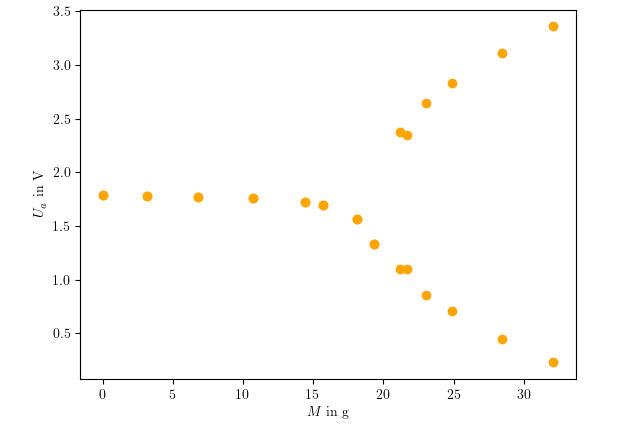
\includegraphics[scale=0.5]{BifurkationMass.png}
    \captionof{figure}{Bifurkationsdiagramm in Abhängigkeit der Masse}
    \label{image:bifu}
\end{center}
Um die kritische Masse $M_k$ zu bestimmen, wird die Differenz $\delta U_a=U_{a,l}-U_{a,r}$ bestimmt und diese quadriert, also $(\delta U_a)^2$. Der Fehler ergibt sich dann aus dem Fehlerfortpflanzungsgesetz, wobei der Ablesefehler $s_a$ auch gleichzeitig als Restfehler $s_r$ abgeschätzt wird. Daraus folgt:
\begin{center}
    \begin{tabular}{r|cccc}
        $M$ [g] &  $U_{a,l}$ [V] &  $U_{a,r}$ [V] &  $s_{U_a}$ [V] &  $(\Delta U_a)^2$ [V] \\
        \hline
         0.00 &  1.78606 &  1.78606 &  0.00005 &   0.0000 \\
         3.14 &  1.78046 &  1.78046 &  0.00050 &   0.0000 \\
         6.78 &  1.77300 &  1.77300 &  0.00500 &   0.0000 \\
        10.75 &  1.76000 &  1.76000 &  0.00500 &   0.0000 \\
        14.42 &  1.72000 &  1.72000 &  0.05000 &   0.0000 \\
        15.72 &  1.70000 &  1.70000 &  0.05000 &   0.0000 \\
        18.10 &  1.57000 &  1.57000 &  0.05000 &   0.0000 \\
        19.36 &  1.33000 &  1.33000 &  0.05000 &   0.0000 \\
        21.19 &  1.10000 &  2.38000 &  0.05000 &   1.6384 \\
        21.67 &  1.10000 &  2.35000 &  0.05000 &   1.5625 \\
        23.05 &  0.86000 &  2.65000 &  0.05000 &   3.2041 \\
        24.88 &  0.71000 &  2.83000 &  0.05000 &   4.4944 \\
        28.45 &  0.45000 &  3.11000 &  0.05000 &   7.0756 \\
        32.12 &  0.23000 &  3.36000 &  0.05000 &   9.7969 \\
    \end{tabular}
    \captionof{table}{Messreihe Auslenkung Gleichgewichtslage}
    \label{tab:gleichgewichtslage}
\end{center}
\begin{center}
    \begin{tabular}{ c | cccccccccc }
        {} & 1 & 2 & 3 &4 &5 &6 &7 &8 &9 &10\\
        \hline
        $T$ [s]&19.14&19.28&18.88&19.18&19.00&18.66&19.12&19.01&19.20&19.29\\
    \end{tabular}
    \captionof{table}{Messreihe Schwingungsdauer}
    \label{tab:schwingung}
\end{center}